\chapter{Methodology}
\label{chapter:methodology}

For the main algorithm of this work from section~\ref{chapter:data_and_algorithm} a few other methods will be used. As they are not the focus of this work we only give a short overview \color{change} in this chapter. \color{black}

\section{Fourier Transformation}
\label{sec:fourier_transformation}

Many applications are concerned with cyclic temporal data. Examples are sound waves or EEG data. This data can be represented as a function of amplitude over time. Most of the time we are not interested in the amplitude at a specific point in time, as a temporal shift would represent very similar information. Such a shift is demonstrated in figure~\ref{fig:tempoal_shift}.

\begin{figure}
	\centering
	
	\begin{subfigure}[b]{\textwidth}
		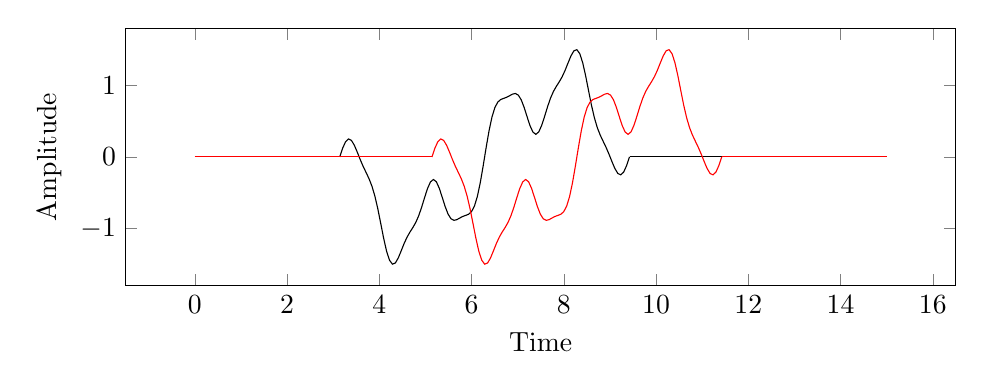
\begin{tikzpicture}
			\begin{axis}[xlabel=Time, ylabel=Amplitude, width=\textwidth, height=0.4\textwidth]
				\addplot+ [domain=0:pi, samples=100, no marks, color=black, style=solid]{0};
				\addplot+ [domain=pi:3*pi, samples=100, no marks, color=black, style=solid]{sin(deg(x)) + 0.5*sin(deg(4*x)) + 0.1*sin(deg(10*x))};
				\addplot+ [domain=3*pi:15, samples=100, no marks, color=black, style=solid]{0};
				
				\addplot+ [domain=0:pi+2, samples=100, no marks, color=red, style=solid]{0};
				\addplot+ [domain=pi+2:3*pi+2, samples=100, no marks, color=red, style=solid]{sin(deg(x-2)) + 0.5*sin(deg(4*(x-2))) + 0.1*sin(deg(10*(x-2)))};section
				\addplot+ [domain=3*pi+2:15, samples=100, no marks, color=red, style=solid]{0};
			\end{axis}
		\end{tikzpicture}
	\end{subfigure}
	
	\caption{Two signals that differ by a temporal shift.}
	\label{fig:tempoal_shift}
\end{figure}

As the function of sound waves or EEG data is cyclic we might be interested in a decomposition into simple cyclic function, such as $\sin$. We can then analyze the most prominent frequencies and their respective amplitudes. This gives a representation of the data, that can be easier to interpret.

We describe one approach to achieve this representation as a weighted sum of $\sin$ functions, called Fast Fourier Transformation (FFT), in algorithm~\ref{alg:fft}.
Figure~\ref{fig:example_fft} shows an example input and output of the FFT algorithm.

\begin{algorithm}
	\caption{Fast Fourier Transformation}\label{alg:fft}
	\begin{algorithmic}
		\Function{FFT}{$x$, $N$, $s$}
			\If{$N$ = $1$}
				\State $X_0 \gets x_0$
			\Else
				\State $X_{0, ..., N/2-1} \gets FFT(x, N/2, 2s)$
				\State $X_{N/2, ..., N-1} \gets FFT(x+s, N/2, 2s)$
				\For{$k=0$ to $N/2-1$}
					\State $p \gets X_k$
					\State $q \gets \exp(-2\pi i/N k) X_{k+N/2}$
					\State $X_k \gets p + q$
					\State $X_{k+N/2} \gets p - q$
				\EndFor
			\EndIf
			\State \Return $X_{0, ..., N-1}$
		\EndFunction
	\end{algorithmic}
\end{algorithm}

\begin{figure}
	\centering
	
	\begin{subfigure}[b]{\textwidth}
		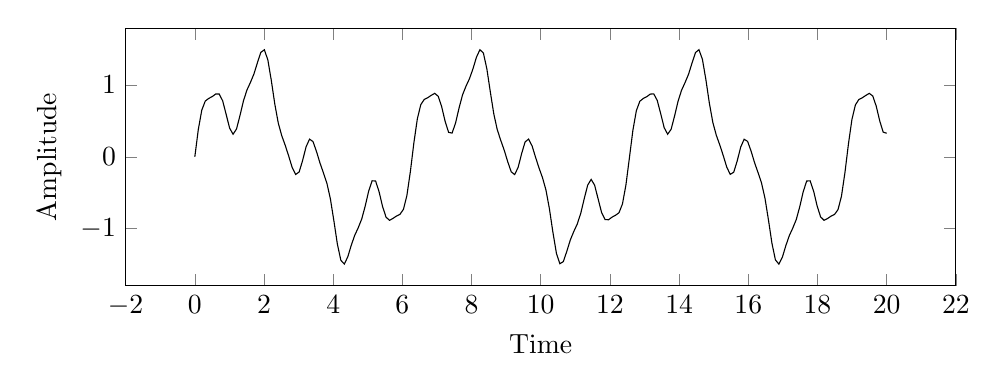
\begin{tikzpicture}
			\begin{axis}[xlabel=Time, ylabel=Amplitude, width=\textwidth, height=0.4\textwidth]
				\addplot+ [domain=0:20, samples=200, no marks, color=black]{sin(deg(x)) + 0.5*sin(deg(4*x)) + 0.1*sin(deg(10*x))};
			\end{axis}
		\end{tikzpicture}
	\end{subfigure}
	\vskip\baselineskip
	\begin{subfigure}[b]{\textwidth}
		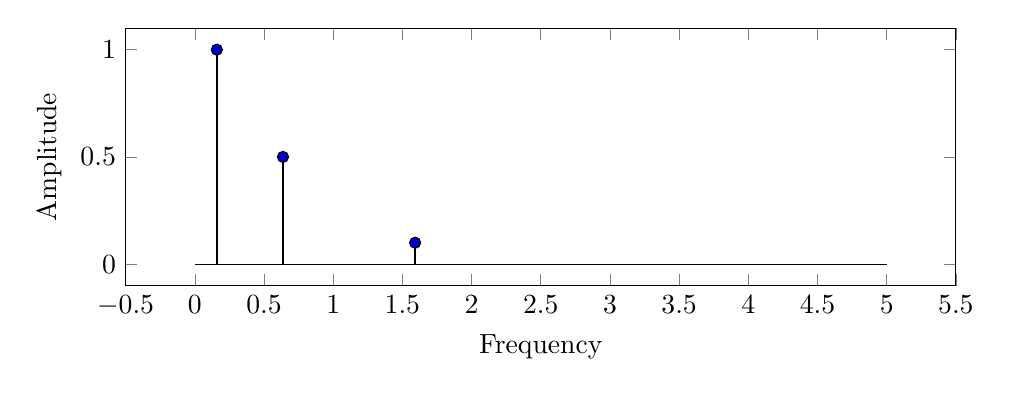
\begin{tikzpicture}
			\begin{axis}[xlabel=Frequency, ylabel=Amplitude, width=\textwidth, height=0.4\textwidth]
				\addplot+ [mark=*, only marks, ybar, bar width=0.5pt, color=black] coordinates {
					(0.159, 1)
					(0.637, 0.5)
					(1.592, 0.1)
				};
				\addplot+ [domain=0:5, samples=100, no marks, color=black]{0};
			\end{axis}
		\end{tikzpicture}
	\end{subfigure}
	
	\caption{A signal composed of different $\sin$ functions and the corresponding FFT output.}
	\label{fig:example_fft}
\end{figure}

\newpage

\section{Classification}
\label{sec:classification}

As the classification algorithm is not the main focus of this work, we decided to go with a simple one.

In classification the objective is to find assignments between data points and categories. In our context we are interested in finding an assignment which closely matches some already categorized data. One simple approach to this problem is the $k$-nearest-neighbors algorithm (KNN).

For data that can be represented in $\mathbbm{R}^m$ and $l$ categories the pseudo code is shown in algorithm~\ref{alg:k_nearest_neighbors}.

\begin{algorithm}
	\caption{$k$ Nearest Neighbors}\label{alg:k_nearest_neighbors}
	\begin{algorithmic}
		\Require data points $(p_i)_{i \in \mathbbm{N}} \in \mathbbm{R}^{m}$, categories $(c_i)_{i \in \mathbbm{N}}, c_i \in \{0, 1, ..., l\} \forall i \in \mathbbm{N}$,
		
		point $x \in \mathbbm{R}^{m}$, $k \in \mathbbm{N}$
		\State Calculate the distance between each point $p_i$ and $x$
		\State Take the $k$ data points with the smallest distance to $x$
		\State \Return the category that most of the $k$ points are assigned
	\end{algorithmic}
\end{algorithm}

If there are significantly more data points in a certain category KNN can be dominated by these categories. As there are more points in the category, they are statistically more common in the $k$ nearest, which leads to $k$-nearest-neighbor giving bad results.

Variations of KNN are achieved by applying a weight to the data points. The weight can depend on the distance between the points.

This algorithm is slow for big datasets as for each point the distance to $x$ has to be calculated. One possibility to reduce calculation time is to partition the space into smaller chunks. Then the loop only has to be over data points lying in the same or close chunks as the point we are interested in.

Figure~\ref{fig:k_nearest_neighbors} shows a graphical representation of the algorithm for points in $\mathbbm{R}^2$ and ${k=10}$.

\begin{figure}
	\centering
	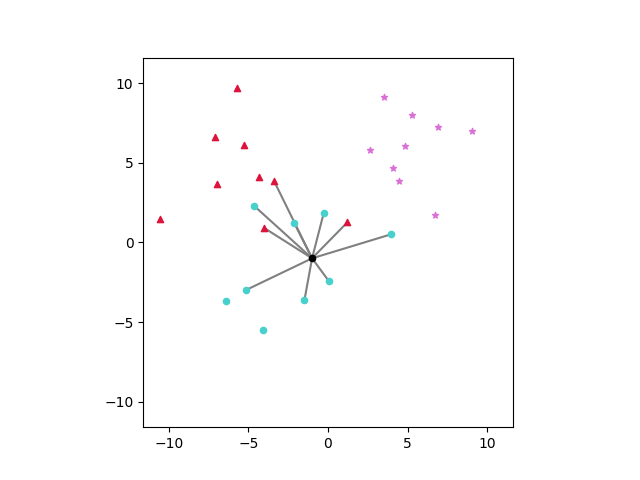
\includegraphics[width=0.45\linewidth]{figs/k_nearest_neighbors}
	\caption{Data points in three categories are given. The black point is classified as a blue, circular point by the k-nearest-neighbors algorithm for $k=10$.}
	\label{fig:k_nearest_neighbors}
\end{figure}